\chapter{Experimental Evaluation} % Or alternatives

Once presented the problem and a proposed model to treat it, some approach is required to test the feasibility of the ideas within this project.
With this in mind, and given the practical interest of the problem, an experimental methodology is proposed, using the library example from section \ref{sec_Library}, to gradually treat the problem and get closer to the applicability of the ideas in real situations.



%In this case, the proposed experimental environment is the library setting described in section \ref{sec_Library} with some simplifications and extensions to emphasize particular parts of the problem.
%By these means, the problem can be divided in smaller

\section{Library Example}

The library setting, presented in section \ref{sec_Library}, provides a good testing environment.
It has some desired qualities for experimentation, principally, a bounded space and a compact set of activities.
%Now, some incremental












If we reuse the library example from chapter 1, it would be worthy to show how the presented approach applies to that problem.
With this in mind, let's first make a simplification of the example.

In Figure \ref{fig:ex_library} is presented a \textit{linear} library. 
It has five connected and consecutive regions: (A) main entrance, (B) printing area, (C) reception, (D) bookshelf and (E) common area.
In this simplified world a person and a robot can move linearly to any region, and they don't obstruct each other.
An activity is performed by a person by visiting regions in a proper order and spending \textit{enough} time on each of them, these intervals are considered within the activity representation.
The challenge here is to recognize the activities of the person

\begin{figure}[h]
\centering
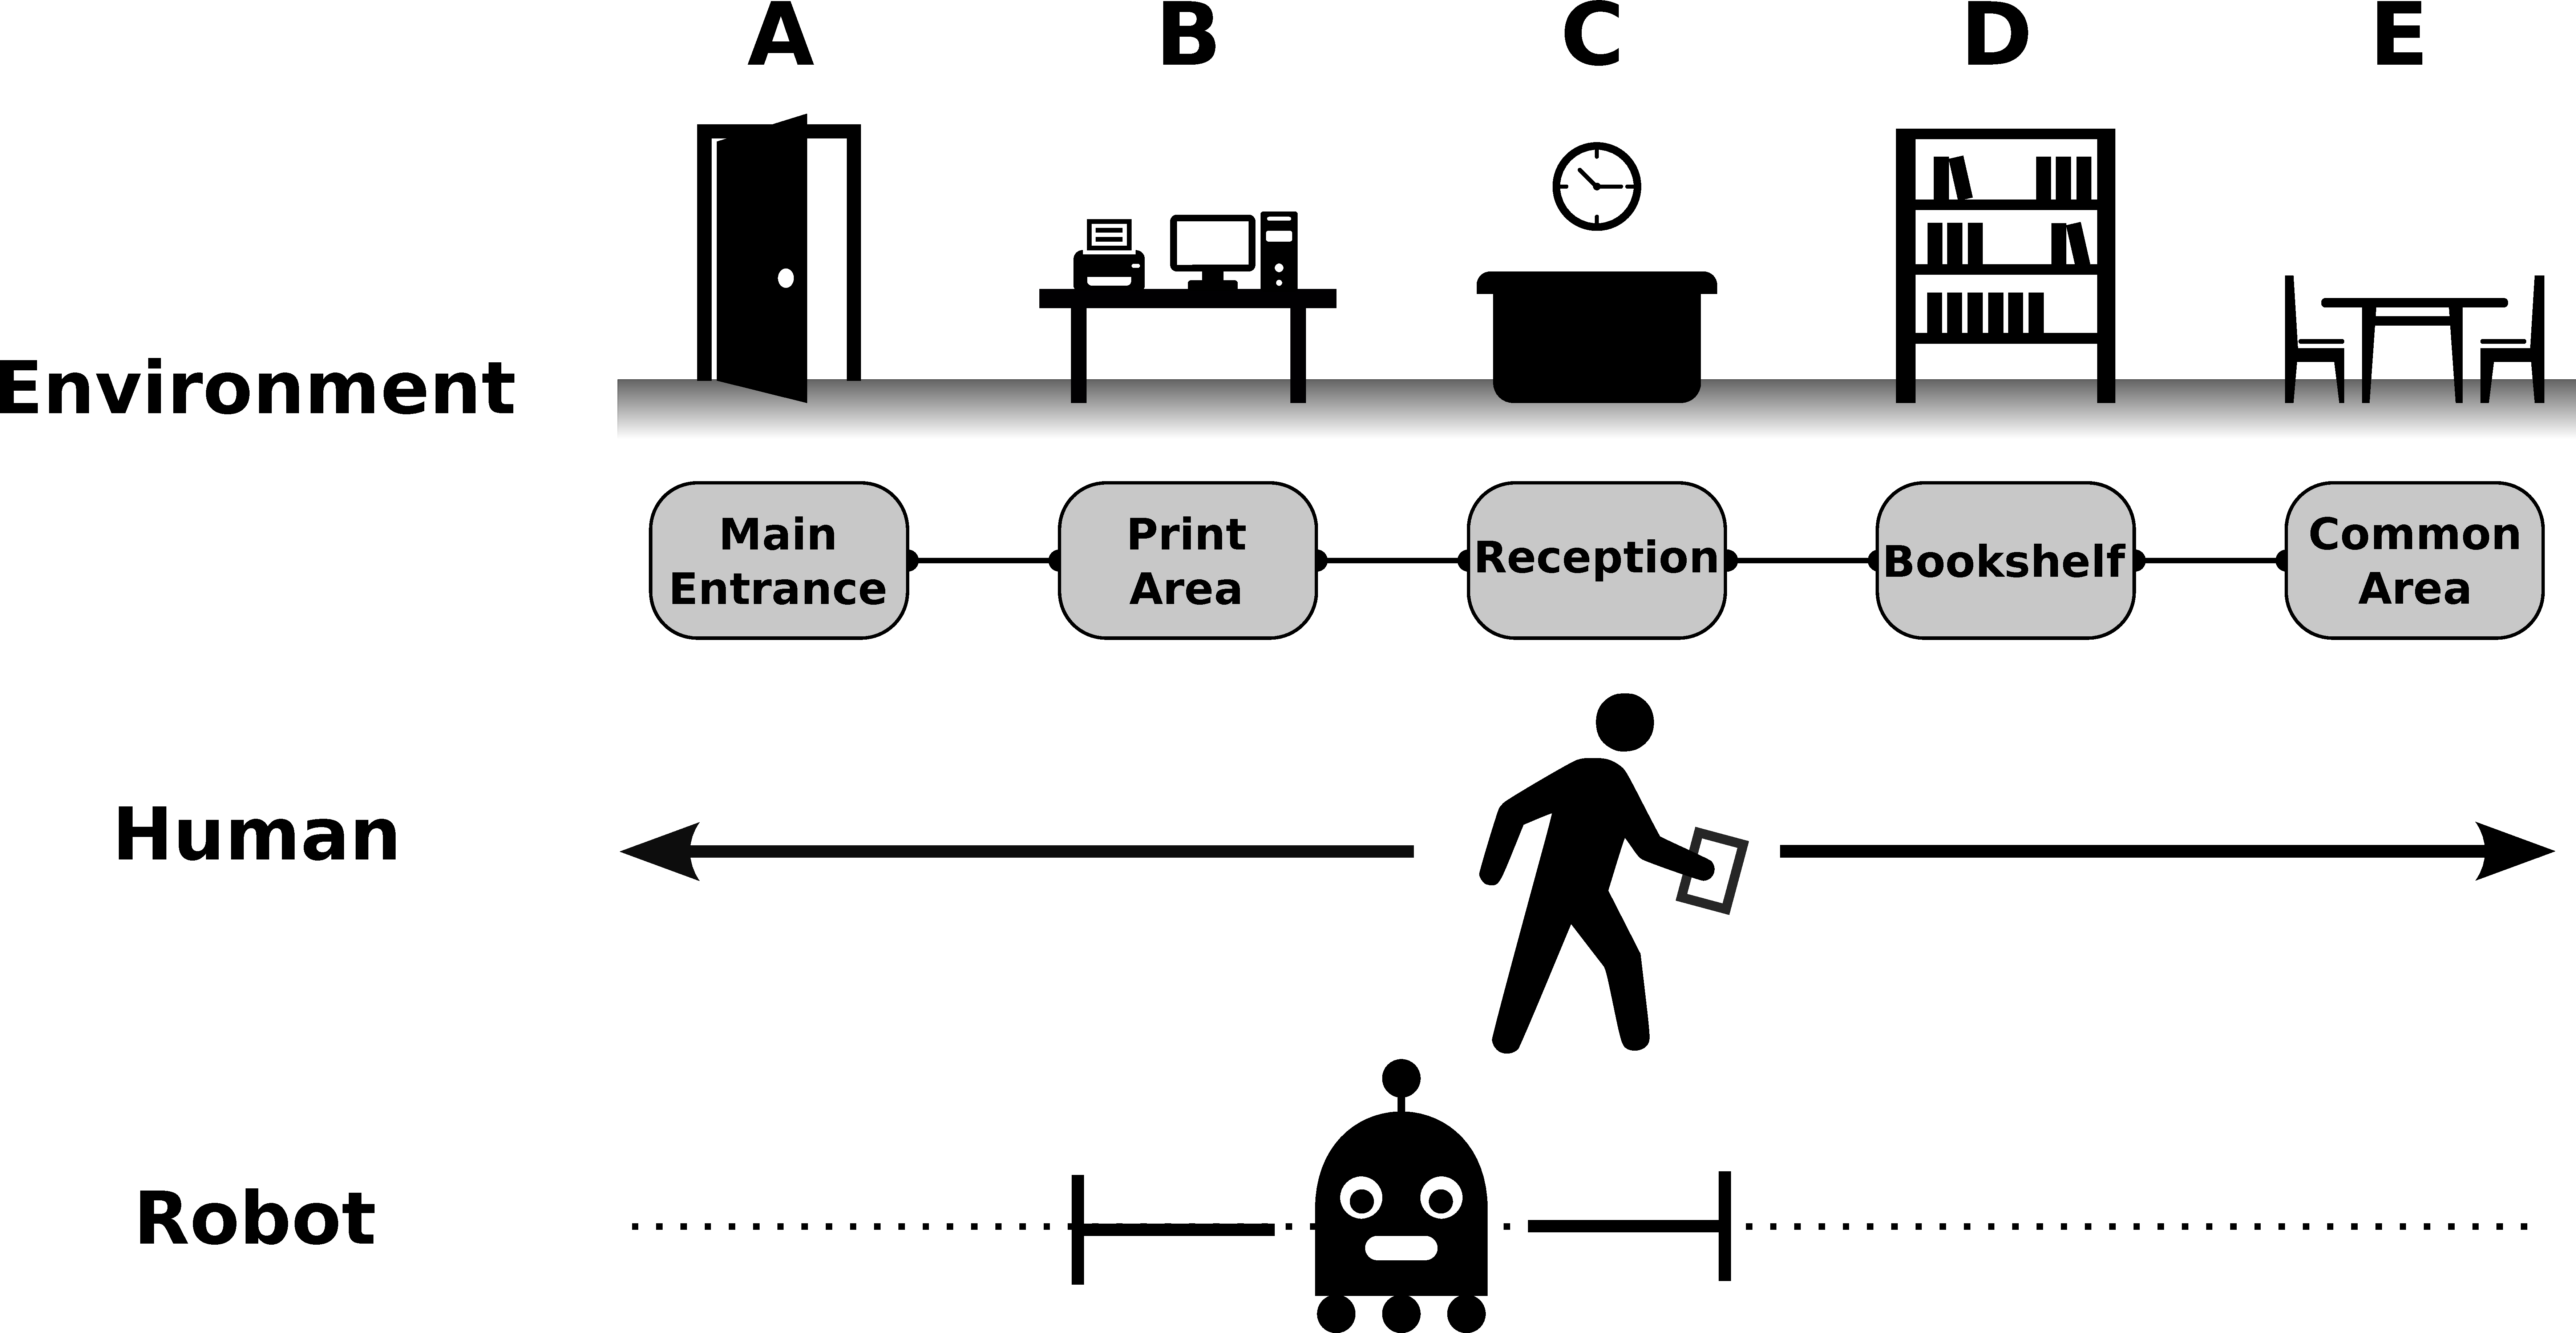
\includegraphics[width=\textwidth]{fig/ex_library.pdf}
\caption{Sensing will be targeting relevant features from humans, objects and from the environment.}
\label{fig:ex_library}
\end{figure}

Some extensions can be induced to this simple world.
\begin{itemize}
\item A robot can have limited sensors, so it will only be able to sense two regions at the same time. 
So, some activeness is required. For example, being observed a person going towards the common area, the robot can move to confirm the position of the person.
\item Handling multiple subjects in the scene, complicates the problem. The robot won't be able to observe all of them, but may try to maximize the observations and after labelling some individuals may go back and sense the rest of the subjects.
\item Object recognition can be induced to disambiguate activities. For example, two activities with the same region description can have an additional parameter regarding the presence of an object. In these cases, a robot can go an confirm the presence or absence of the object to discriminate its hypotheses. 
\end{itemize} 


However, let's use now just the simple case with only one subject and with the activities defined just regarding the visited regions.
The following activities can be defined:

\begin{description}
\item[print]$B$ 
\item[study]$D \rightarrow E$
\item[bookLoan]$D \rightarrow C$
\item[bookRetrieval]$C$
\item[requestAssistance]$C$
\end{description}

%TODO %TODO %TODO Complete the example.







\section{Final evaluation}

First, this project makes emphasis in the use of a robot, which has some evident limitations.
Sensors are constrained to defined ranges and the thrown data usually presents noise.
Actuators also present inaccuracies and time-delayed responses.
Processing capabilities are also limited in a robot, so the amount of data collected with a robot should be minimized and processed efficiently whenever is possible.
%This is, however, the current state in robotics and this is considered by considering sensor models, 

Regarding ASP, here is used for knowledge representation and reasoning purposes. 
It can also provide a path to plan actions for the robot.
ASP should be used with reserve as it is used to model combinatorial NP-hard problems.
With this in mind, should be noted that ASP implementations are limited in efficiency and the modelled problems can grow very easily.
This is considered in this project by restricting the domain application (to a library), the amount and granularity of the descriptions for activities, objects and places. 

The idea is to go from a simple case to more complex, general and realistic cases. 
An experimental approach is going to be followed, so it an important question how are the results going to be evaluated.
Two possibilities are considered now.

First, to compare our library setting with other techniques. 
This is, to implement other approach, run it in the same conditions than the one developed in this project, and compare results.
This have the advantage than the experiments can be in control and many situations can be explored (e.g. different starting points, different environmental conditions, different activities, objects, etc.).

The second possibility is to use a dataset for activity recognition, as \citep{Tenorth2009_TUMKData}, and compare our ASP-based approach with other ones.
This has the advantage that the results to compare are already available as well as the sensory data.
However, the disadvantage is that there are no datasets for activity recognition with robots. 
So the way to proceed would be only to compare the stand-alone activity recognition system with ASP.



% Main parts of the problem

% A - Scene decomposition (locations, objects, persons)
%   > from observations to scene reconstruction

% B - 

% B - Representation 
% Modelling in space (QSR)
% Modelling in time (QSTR)











